\section{Quickstart}
\label{quickstart}

\subsection{Eintragen der Lehrveranstaltungsnote}

Das Benotungstool im CIS des Technikum Wien ist als Schnittstelle zwischen LektorIn und AssistentIn das zentrale Werkzeug f�r die Notenverwaltung.\\

\noindent
{\bf Bitte verwenden Sie das Tool zum Eintragen der Lehrveranstaltungsnote:}

\begin{enumerate}
\item W�hlen Sie unter \url{https://cis.technikum-wien.at} -$>$ Mein Cis -$>$ Meine LV eine Lehrveranstaltung aus. Auf der �bersichtsseite klicken Sie das Symbol 'Benotungstool' (s. Abb. \ref{uebersicht_lv}, S. \pageref{uebersicht_lv})
\item Klicken Sie nun auf im linken oberen Seitenbereich auf 'Lehrveranstaltung benoten'
\item Tragen Sie nun Noten ein und �bernehmen Sie diese mit dem '-$>$' - Knopf
(1)
\item Wenn Sie alle Noten eingetragen haben, die  Sie zu diesem Zeitpunkt
eintragen wollen (Sie k�nnen jederzeit Noten nachtragen!) k�nnen Sie diese
�ber den Knopf 'Freigabe' (im Tabellenkopf) f�r die AssistentIn freigeben.
(2)\\ 
ACHTUNG: aus Gr�nden der erh�hten Sicherheit ist bei der Freigabe der Noten
die Eingabe Ihres Passwortes erforderlich.\footnote{Es handelt sich dabei um Ihr
TW-Passwort, mit dem sie sich auch auf der CIS-Seite authentifizieren oder auf
unseren Rechnern einloggen}
\item Fertig!
\end{enumerate}


\begin{figure}[ht]
\begin{center}
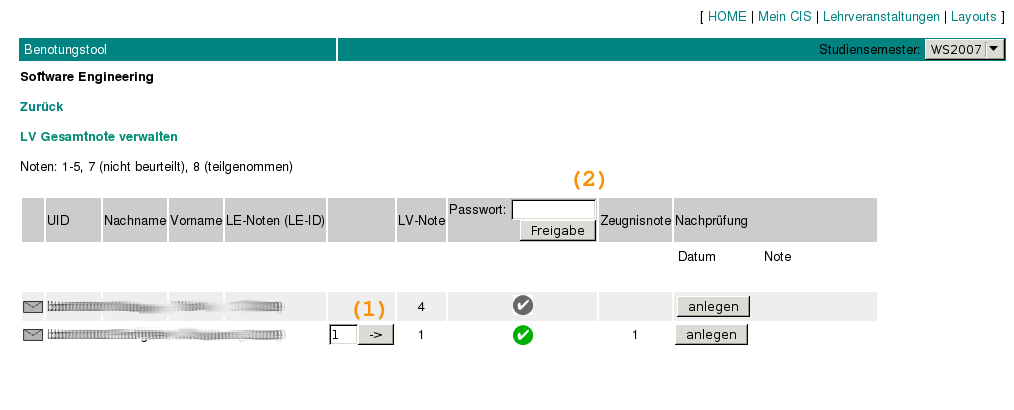
\includegraphics[width=1.0\textwidth]{benotungstool_benotung_lv.png}
\end{center}
\caption{Benotung LV}\label{benotung_lv_quick}
\end{figure}

\noindent
Weitere Informationen s. Kap. \ref{gesamtnote} auf S. \pageref{gesamtnote}\\




